

\documentclass[12pt,]{article}
\usepackage{zed-csp,graphicx,color}%from
\pagenumbering{roman}
\begin{document}
\begin{titlepage}
\centerline{Implementation of indigenous Electronic Medical Record System to\\}
\centerline{ Facilitate Care of Sickle cell Disease Patients in Uganda.\\}
\paragraph*{•}
\centerline{  Prepared by:  Nakyewa irene 16/U/851 216000677.\\}
\centerline{DATE: $February,24^{th},2018$\\}
\centerline{Supervisor: Ernest Mwebaze\\}

\paragraph*{•}
\paragraph*{•}
  \centerline{Data Collection Concept}
\date{\today}
\end{titlepage}

\newpage



\pagenumbering{arabic}
\section{Introduction}
Sickle Cell Disease
(SCD), which causes a wide range of severe and even life threatening consequences, is caused by a single misspelling in DNA instructions for hemoglobin, protein vital  for carrying  oxygen in blood .As a result of this mutation, individuals with SCD experience lifelong complications including anemia, infections, stroke and many and premature death. These debilitating symptoms and the complex treatment needs of people living with often limit their education, carrier opportunities and quantity of life. Sickle cell disease (SCD) is prevalent in Uganda central Uganda including mainly some eastern parts( karamoja).Screening for (SCD) is carried out by the government of Uganda . 
\section{Background}
Sickle cell Disease(SCD) is a genetic blood disorder affecting red blood cells, with high mordability rates .Over the past years, great advances have been made in the understanding and treatment of sickle cell disease .This disease is caused by a single mutation, that has advanced the field of modern human molecular biology ,many discoveries have been made and some some treatments developed . The Sickle cell support organizations have recognized SCD as a global public health concern, and the The sickle cell prevention organisations recommends that 50% pf member states will have established SCD control  programs by 2018
This Paper presents an integrative review of the references related to SCD among children below the age of 20 in Uganda ,This review focuses on the incidence ,prevalence,mordabity,and mortality:current practices and challenges related to screening ,diagnosis and treatment :and recommendations for this practice, Policy ,and research to improve health outcomes of children with SCD in Uganda.
There have been significant improvements in the mordability and mortality rates for children with SCD in high resource regions due to factors such as early diagnosis through newborn screening programs and comprehensive care programs 
\begin{figure}
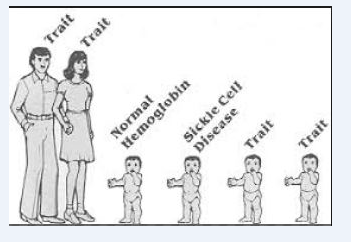
\includegraphics[width=\linewidth]{intro.png}
\caption{about sickle cell}
\end{figure}
\newpage
\newpage
\section{Problem Statement}
Every Year few million children in Uganda have suckle cell disease ,most whom may not live beyond adoloscenece.even though the health organizations have  recognized size of the problems and its increasing burden ,very little have been done soffer Sickle cell is curable and the trait can be prevented but only a minority of the patients have access to appropriate care .A lack of trained personnel and a financial resources are these patient’s major barriers to healthy life.



\section{Objectives}
\subsection{Main objectives}
\begin{itemize}
\item To develop an Electronic Medical Record system(digital version of paper chart that contains patients  medical history) to facilite sickle cell patients in Uganda as well as Africa that can keep track of patients information .The Electronic Medical report system can help the doctors practice better medicine and improve bottom line.
Specific objectives
\item To decrease the number of Hospital phone calls regarding prescriptions.
\item To decrease transcription turnaround time and reduce transcription cost
\item To improve the quality of care of sickle cell patients to the  waiting room time patients
\item To collect and analyze data from patients, doctors, and hospital managers
\end{itemize}

\section{Scope}
The research study is aimed at sickle cell patients in uganda(Eastern and western parts) and to generate an electronic medical record system  for the wellbeing and welfare of sickle cell patients .The future scope of  study will be supportive and beneficial to government to have a database on the current awareness of youth about disease


\section{Research Significance}
The study is important because it aims at developing an Electronic Medical Record system that can be used improve the quality care and enhance performance measurement
\section{Literature review}
Sickle -cell anemia (SCA) ,is a heredaory disorder , that results from singlr point mutation in haemoglobin B chain by substitution of valine in state of glutamic acd at 6 position.In 1910 ,Herrick described an anemia characterized by bizarre, sickle-shaped cells.The role of deoxygenaton was discovered in the 1920’s by Hahn and Gillespie.The research survey on sickle cell disease (SCD) was basically done in Uganda ,Africa and SCA is estimated to contribute equivalent of 5% of under -five deaths, with up to 16% in some countries such as Nigeria .There are a number of studies till date performed on the sickle cell anemia by  alloptuc of alternative medicine .In autosomal disorder where there is no cure than creating awareness in the youths and making positive impact into the mind of tribal people can atleast be helpful in motivating people for utilizing patient cancelling ,genetic and premarital neonal screening facilities provided by health care system. The first survey on sickle cell done in Uganda in 1949, reported the district of Bundibugyo in Western Uganda to have the highest sickle cell trait(SCT) Prevelance (45%).This is believed to be the highest in the world wide. According to the same survey, the prevalence of SCT in districts of Mbale  and Sironko in East was 20-28%whlist the districts of Mbarara and Ntungamo in the west.


\subsection{The symptoms of sickle cell Anemia:}
The following is symptoms and complications associated with sickle cell anemia each patient may experience different symptoms which may include: The most common symptoms of anemia is fatigue (feeling tired or weak), other signs and symptoms may include; Shortness of breath, Diziness,headaches,coldness in Hands and feet, paler or normal and many others
\begin{figure}
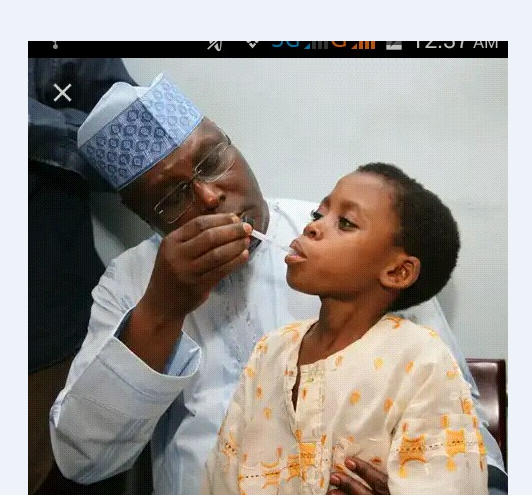
\includegraphics[width=\linewidth]{sickle 1.png}
\caption{Patient's Current Status}
\end{figure}
\newpage
\section{Methodology}
The data process will mainly rely on both interviews and questioners for data collection and analysis, this will help collect sufficient information. The data collected during such activities will be managed using ODK., which later be uploaded to the ODK aggregate server to carry out all the required analysis. Different kinds of data including images and some videos will be collected these include:Patient name, recent photo, Place of residence, Age, Health Records, Test results, Appointments
\subsection{Collection of data through screening program}
In Uganda, screening program mainly is carried out in school to children and they are screened through hemoglobin solubility test to identify presence of sickle hemoglobin. For children found positive for hemoglobin solubility test, blood samples are sent to central laboratory at the institute for hemoglobin electrophoresis test to identify genotype status i.e sickle cell carrier(AS) and sickle cell disease patient 

\section{References}
International Alliance of Patient’s organizations patientorganisations.org
www.Human-Medicare Supplimaent.com/Gaplnurance/HumanMedicare
https://www.medicare.gov








\end{document}






